\documentclass{beamer}
\usetheme[color=ACMblue]{ACMNew}
\usepackage{beamernotes}
\usepackage{algpseudocodex}
\usepackage{lipsum}
\usepackage{minted}
\usepackage{array}
\usepackage{tikz}
\usepackage{amsmath}
\usepackage{mathtools}
\usepackage{xcolor}
\usetikzlibrary {automata,positioning,calc,shapes.geometric} 
\usemintedstyle{manni}
\pdfcompresslevel=9
\pdfobjcompresslevel=3

\title[ACM fun]{CS 374A Final Review}
\subtitle{The Multiple-Choice Final Boss of Algorithms}
\author{ACM @ UIUC}
% \institute{The Mental Institute}  
\date{November 3, 2024}


\begin{document}

\begin{frame}
  \titlepage
\end{frame}
\bnote{This generates notes for pdfpc. These notes also appear
  on the handout/article versions.}

\begin{frame}[t]{Disclaimers and Logistics}
  \begin{itemize}
  \item \alert{Disclaimer:} Some of us are CAs, but we have not seen the exam. We have no idea what the questions are. However, we've taken the course and reviewed Kani's previous exams, so we have \alert{suspicions} as to what the questions will be like.
  \item This review session is being recorded. Recordings and slides will be distributed on EdStem after the end.
  \item \alert{Agenda:} We'll quickly review all topics likely to be covered, then go through a practice exam, then review individual topics by request.
  \begin{itemize}
      \item Questions are designed to be written in the same style as Kani's previous exams but to be \textit{slightly} harder, so don't worry if you don't get everything right away!
  \end{itemize}
  \item Please let us know if we're going too fast/slow, not speaking loud enough/speaking too loud, etc.
  \item If you have a question anytime during the review session, please ask! Someone else almost surely has a similar question.
  \item We'll provide a feedback form at the end of the session.
  \end{itemize}
\end{frame}

\begin{frame}
\frametitle{Table of Contents}
\tableofcontents
\end{frame}

\section{Models of Computation}

\begin{frame}[t]{Induction}
    \begin{exampleblock}{Template}
    Let $x$ be an \textit{arbitrary} <OBJECT>. Assume for all $k$ s.t. $k$ is smaller than $x$ (by <ORDERING PROPERTY>), that $P(k)$ holds.

    \vspace{.5cm}
    
    If $x =$ <MINIMAL OBJECT>, then $\dotsc$, so $P(x)$ holds

    \vspace{.5cm}

    If $x \neq$ <MINIMAL OBJECT>, then $\dotsc$, so by IH, $\dotsc$, so $P(x)$ holds.

    \vspace{.5cm}

    Thus, in all cases, $P(x)$ holds.
    \end{exampleblock}
    \vspace{.7 cm}
    \pause Some tips:
    \begin{itemize}
        \item \alert{Always use strong induction}. All weak inductive proofs can be re-written to use strong induction with minimal changes, and the extra assumption can make your life significantly easier.
        \item \alert{Write out your IH, base case, and inductive step out explicitly.} Doing so will help you avoid getting confused, and will help you avoid losing points.
        \item If you're performing induction on a recursive definition (strings, CFLs, etc.), generally, your inductive step will consist of one step of the recursion, and then will use IH.
    \end{itemize}
\end{frame}

\subsection{Regularity}

\begin{frame}[t]{Regular Languages/Expressions}
    \begin{itemize}
        \item Built inductively on 3 operations:
        \begin{itemize}
            \item \pause $+$ is the union operator. $L(r_1 + r_2) = L(r_1) \cup L(r_2)$
            \item \pause $*$ is the Kleene star. $L(r_1^*) = L(r_1)^*$
            \item \pause $()$ are used to group expressions
            \item \pause (implicit) concatenation operator: $L(r_1r_2) = \{xy : x \in L_1, y \in L_2\}$
        \end{itemize}
        \item \pause Closed under Union ($\cup$), intersection ($\cap$), concatenation ($\cdot$), kleene star (${}^*$), complement ($^C$), set difference ($\setminus$), and reverse (${}^R$)
        \begin{itemize}
            \item \pause ... but only finitely many applications of these operations
        \end{itemize}
        \item \pause If trying to guess whether or not a language is regular, think about memory. When processing a string through a DFA, you only need to know which state you're currently in, and do not need to look forwards/backwards in the string.
        \begin{itemize}
            \item Implementing a DFA/NFA in code only requires $O(1)$ memory
            \item If your checker program needs to count something without bound, the language you're checking isn't regular.
        \end{itemize}
        \item \pause \alert{Regex Design Tips:} If you don't know where to start, try giving examples for strings that are in the language and strings that aren't. Look for patterns and try to build components around those patterns, then combine into something that represents the full language. Make sure to test and modify for edge cases. Explain, in English, each part of your regular expression with a short sentence. Does the explanation match the language?
    \end{itemize}
\end{frame}

\begin{frame}[t]{DFAs/NFAs}
    \begin{itemize}
        \item DFAs defined by \textit{state set} $Q$, \textit{accepting set} $A \subseteq Q$, \textit{input alphabet} $\Sigma$, \textit{start state} $s \in Q$, and \textit{transition function} $\delta: Q \times\Sigma \rightarrow Q$
        \item NFAs allow for ``trying'' multiple transitions at the same time or transitioning without reading in ($\epsilon$-transitions), accepts if there is a path to an accepting state. Transition function thereby changes to $\delta: Q \times(\Sigma \cup\{\epsilon\}) \rightarrow 2^Q$
        \begin{itemize}
            \item Power-set construction to convert from NFA to DFA- in theory exponential-time but used in practice.
        \end{itemize}
        \item \alert{Tips for creating DFA/NFAs}: Break down your language into smaller patterns, and figure out what you need to store as state for each part. Make sure you clearly define all components. A drawing or transition table is just as valid as a $(Q,A,\Sigma, s, \delta)$ definition. \pause
        \begin{block}{Product Constructions}
            Given some languages $L_1, \dots, L_n$ we want a DFA that accepts strings $w$ satisfying $f(w \in L_1,\dots,w \in L_n)$ where $f$ is some logical function. Create a DFA/NFA for $L$ using the following \textit{rough} format:
            \begin{itemize}
                \item $Q = Q_1 \times \cdots \times Q_n$
                \item $\delta'(q_1,\dots,q_n) = (\delta_1(q_1),\dots,\delta_2(q_2))$
                \item $s = (s_1,\dots,s_n)$
                \item $A' = \{\text{convert $f$ into a set expression}\}$
            \end{itemize}
        \end{block}
    \end{itemize}
\end{frame}

\subsection{Irregularity and Transformations}

\begin{frame}[t]{Fooling Sets}
    \begin{itemize}
        \item DFAs only care about which state you're in, and not how you got there
        \begin{itemize}
            \item If two strings result in the same DFA state, any additional suffix added to both will also result in both strings being in the same state.
            \item \pause Thus, if we have $w, w'$, and we know that there exists a \alert{distinguishing suffix} $z$ s.t. $wz \in L, w'z \not\in L$, then $w, w'$ must be in \textit{different} states for \textit{any} DFA that accepts $L$ 
        \end{itemize}
        \item\pause A \alert{fooling set} is a set of strings where there exists a distinguishing suffix between every pair of strings
        \item Myhill-Nerode: min DFA size = max fooling set size
        \begin{itemize}
            \item \pause Thus, languages with infinite fooling sets are \textit{not} regular
        \end{itemize}
        \item \pause If you see the need to keep track of something without bound, you can create a fooling set around the part where you count up.
        \item \pause \alert{If you see divisibility, think primes!} All primes are coprime, so primality provides for an infinite set with easier construction of distinguishing suffixes.
        \item \pause If you're using strings of the form $1^k, 0^p$, etc. when sampling elements of your fooling set $a^i, a^j$, it's completely fine to assume WLOG that $j > i$, but nothing about the underlying structure of $i$ and $j$. If you want to put in such a restriction, you should instead restrict your fooling set further.
    \end{itemize}
\end{frame}

\begin{frame}[t]{Language Transforms}
    \begin{itemize}
        \item Used to prove that regularity is closed under some function $f$ (if $L$ is regular, then $f(L)$ is regular).
        \item \alert{General Format:} Given a DFA $M$ that accepts $L$, create an NFA $M'$ that accepts $f(L)$.
        \item \pause \alert{General Strategy:} Apply non-determinism to guess the future behavior of the DFA that you want to simulate.\pause
        \vspace{1 cm}
        \begin{alertblock}{Make sure you're going in the right direction!}
            If you see the format $f(L) = \{k(w) : w \in L\}$, your modified NFA should be trying to \textit{undo} $k$, while if you see the format $f(L) = \{w : k(w) \in L\}$, your modified NFA should be trying to \textit{apply} $k$. Mixing these up is the most common mistake we see on homeworks/exams.

            \vspace{.25cm}
            
            In some cases, only one direction is possible. For example, $\texttt{un-palin}(L): \{w : ww^R \in L\}$ has a transformation construction, but $\texttt{palin}(L) = \{ww^R: w \in L\}$ is irregular for some $L$.
        \end{alertblock}
    \end{itemize}
\end{frame}

\subsection{Context-Free Grammars}

\begin{frame}[t]{Context-Free Languages/Grammars}
    \begin{itemize}
        \item Formally, a context-free grammar is defined by \textit{nonterminals/variables} $V$, \textit{terminals/symbols} $T$, \textit{productions} $P$, 
        and the \textit{start symbol} $S$. Each production rule in $P$ looks like $A \to \alpha$, where $A \in V$ and $\alpha \in (V \cup T)^*$.

        \item \pause For example, consider $V = \{S\}, T=\{0,1\}, P=\{S \to \epsilon, S \to 0S1 \}$. (You can abbreviate this to $P=\{S \to \epsilon \mid 0S1 \}$.) What language is this?

        \begin{exampleblock}{Intuition}
            CFGs "build" strings, going from the outside in; you can choose rules to add characters on the left/right.
            
            Alternatively, CFGs "peel back" strings, removing characters from the left/right until nothing is left.
        \end{exampleblock}

        \item \pause CFLs only closed under union, kleene star, and concatenation. CFLs are \textit{not} closed under intersection or complement.

    \end{itemize}

    \pause \begin{center}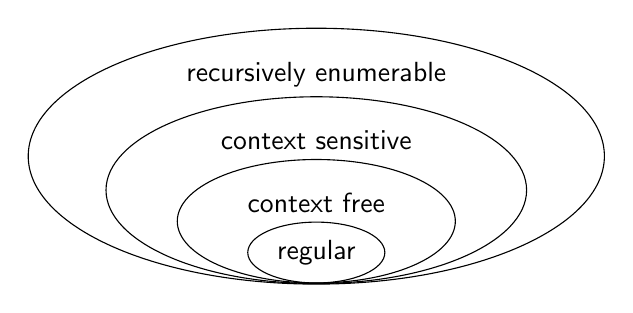
\begin{tikzpicture}[font=\sffamily,breathe dist/.initial=2ex]
    \foreach \X [count=\Y,remember=\Y as \LastY] in 
    {regular,context free,context sensitive,recursively enumerable}
     {\ifnum\Y=1
      \node[ellipse,draw,outer sep=0pt] (F-\Y) {\X};
     \else
      \node[anchor=south] (T-\Y) at (F-\LastY.north) {\X};
      \path let \p1=($([yshift=\pgfkeysvalueof{/tikz/breathe dist}]T-\Y.north)-(F-\LastY.south)$),
      \p2=($(F-1.east)-(F-1.west)$),\p3=($(F-1.north)-(F-1.south)$)
      in ($([yshift=\pgfkeysvalueof{/tikz/breathe dist}]T-\Y.north)!0.5!(F-\LastY.south)$) 
      node[minimum height=\y1,minimum width={\y1*\x2/\y3},
      draw,ellipse,inner sep=0pt] (F-\Y){};
     \fi}
    \end{tikzpicture}\end{center}
\end{frame}

\begin{frame}[t]{Practice Questions I}
\begin{enumerate}
    \item Let $L$ be a regular language. Then, $L \cap \{0^n1^n: n > 0\}$ is$\dotsc$

    \begin{enumerate}[(a)]
        \item always regular
        \item always irregular, but always context-free
        \item sometimes irregular, but always context-free %correct%
        \item sometimes non-context-free
    \end{enumerate}
    
    \pause\item Define $\textsc{coverEvens}(w_1 w_2 \dotsb w_n) =  k_1 k_2 \dotsb k_n$ and $\textsc{coverExponential}(w_1 w_2 \dotsb w_n) =  c_1 c_2 \dotsb c_n$, where $k_i = \begin{cases}
        1 &\text{ if } i \equiv 0 \pmod{2}\\
        w_i &\text{otherwise}
    \end{cases}$ and $c_i = \begin{cases}
        1 &\text{ if } \exists n \in \mathbf{Z} \text{ s.t. } i = 2^n\\
        w_i &\text{otherwise}
    \end{cases}$. 
    
    Which of the following is true?
    \begin{enumerate}[(a)]
        \item If $L$ is a regular language, then $\textsc{coverEvens}(L)$ is regular. %correct%
        \item If $\textsc{coverEvens}(L)$ is a regular language, then $L$ is regular. %subtily wrong%
        \item If $L$ is a regular language, then $\textsc{coverExponential}(L)$ is regular.
        \item If $\textsc{coverExponential}(L)$ is a regular language, then  $L$ is regular.
        \item Exactly two of the above are true
        \item Exactly four of the above are true
    \end{enumerate}
    \pause\item If we instead define $\textsc{UnCoverEvens}(L)$ to be $\{w: \textsc{CoverEvens}(w) \in L\}$, then would $\textsc{UnCoverEvens}(L)$ be regular for all regular $L$?
    \begin{enumerate}[(a)]
        \item Yes %correct%
        \item No
    \end{enumerate}
\end{enumerate}
\end{frame}

\begin{frame}[t]{Practice Questions II}
    \begin{enumerate}
        \setcounter{enumi}{3}
        \item If $L$ is decided by a DFA with $n$ states, then consider the language $L'$ consisting of all strings in $L$ with at most 374 characters removed. Which of the following is true?
        \begin{enumerate}[(a)]
            \item $L'$ can be decided by a DFA with $O(n)$ states
            \item $L'$ can be decided by a DFA whose number of states is polynomial in $n$
            \item $L'$ can be decided by a DFA whose number of states is exponential in $n$
            \item We cannot guarantee that there exists a DFA which decides $L'$
        \end{enumerate}
        \pause\item Consider the language $L$ consisting of the binary representation of all numbers congruent to 173 mod 374.
        \begin{enumerate}[(a)]
            \item $L$ does not have a fooling set.
            \item $L$ has a fooling set of size 173.
            \item $L$ has a fooling set of size 374. %correct%
            \item $L$ has a fooling set of size 375.
            \item $L$ has an infinite fooling set.
        \end{enumerate}
        \pause\item Given a DFA $M$ with $n$ states, the minimum length of a string that $M$ must accept (if $L(M)$ is non-empty) is at most:
            \begin{enumerate}[(a)]
                \item $n$
                \item $n-1$ %Correct%
                \item $2^n$
                \item $2^n-1$
                \item $n^2$
            \end{enumerate}
    \end{enumerate}
\end{frame}
\begin{frame}[t]{Practice Questions III}
    \begin{enumerate}
        \setcounter{enumi}{6}
        \item If $L_1$ is regular and $L_2$ is undecidable, then $L_1\cap L_2$ is:
            \begin{enumerate}[(a)]
                \item Always regular
                \item Always context free
                \item Always undecidable 
                \item Always decidable
                \item Could be decidable or undecidable depending on $L_1$ %Correct%
            \end{enumerate}
        \pause \item Given a language L, which of these is NOT necessarily true if L is context-free?
            \begin{enumerate}[(a)]
                \item $L^*$ is context-free
                \item $L \cup \{\epsilon\}$ is context-free
                \item $L\cap R$ is context-free for any regular language $R$
                \item $L^R$ (reverse of L) is context-free
                \item $\{w\#w \mid w \in L\}$ is context-free %Correct%
            \end{enumerate}
        \pause \item Given a regular expression of length n, the equivalent minimum DFA might have
            \begin{enumerate}
                \item $O(n)$ states
                \item $O(n^2)$ states
                \item $O(2^n)$ states %Correct%
                \item $O(n!)$ states
                \item Always exactly n states
            \end{enumerate}
    \end{enumerate}
\end{frame}


\section{Algorithms}

\begin{frame}[t]{Recursion}
  \begin{itemize}
    \item \alert{Definition:} Reducing the problem to a smaller instance of itself, where eventually we can terminate in a base case.
    \begin{itemize}
        \item Think: If we have a problem of size $n$, we want to continuously reduce to a problem smaller than $n$.
        \item Example: Tower of Hanoi
    \end{itemize}
    \begin{exampleblock}{Template}
        \begin{algorithmic}[1]
                \Procedure{AmazingRecursiveAlgo}{n}
                    \If {$n$ == [some base case]}
                        \State return [value]
                    \Else 
                        \State return \texttt{AmazingRecursiveAlgo}($n-1$)
                    \EndIf
                \EndProcedure
        \end{algorithmic}
        
    \end{exampleblock}
    \item Similar to \alert{induction}!
  \end{itemize}
\end{frame}

\begin{frame}[t]{Recursion: Runtime Analysis}
  \begin{itemize}
    \item \alert{General Form:} $$T(n) = \underbrace{r}_{\mathclap{\text{\# of subproblems}}} \; \cdot \; 
\overbrace{T\left(\frac{n}{c}\right)}^{\mathclap{\text{work at each subproblem}}} 
\; + \; \underbrace{f(n)}_{\mathclap{\text{work at current level}}}$$
    \begin{itemize}
        \item Describes how the amount of work changes between each level of recursion.
        \item We can solve for a \alert{time complexity} that describes the scaling behaviour of the algorithm at hand.
    \end{itemize}

    \pause
    \item \alert{Master's Theorem}
    \begin{block}{Master's Theorem}
        \begin{align*}
            \text{Decreasing: } r \cdot f(n / c) = \kappa \cdot f(n) \text{ where } \kappa < 1 &\implies T(n) = O(f(n)) \\ 
            \text{Equal: } r \cdot f(n / c) = \kappa \cdot f(n) \text{ where } \kappa = 1 &\implies T(n) = O(f(n)\cdot log_{c}{n}) \\
            \text{Increasing: } r \cdot f(n / c) = \kappa \cdot f(n) \text{ where } \kappa > 1 &\implies T(n) = O(n^{\log_{c}{r}})
        \end{align*}
    \end{block}
    \pause
    \begin{itemize}
        \item \alert{Intuition:} If each level contains more work than the level below it, then the root level will dominate. If each level contains the same amount of work, then we have $log_{c}{n}$ levels with $f(n)$ work. If each level contains less work than the work below it, then the leaf nodes will dominate.
    \end{itemize}
  \end{itemize}
\end{frame}

\subsection{Divide and Conquer}
% Mergesort
\begin{frame}[t]{Divide and Conquer Algos: Merge Sort}
    \begin{itemize}
        \item \alert{Purpose:} Sort an arbitrary array.
        \item \alert{Time Complexity}: $O(n \log n)$
        \item \alert{Intuition:} Three phases: (a) split the array in half, (b) sort each side, (c) merge the sorted halves by repeatedly comparing smallest elements on each side not yet inserted.
        \begin{figure}
            \centering
            \includegraphics[width=0.5\linewidth]{mergesort.png}
        \end{figure}
    \end{itemize}
\end{frame}

% Quickselect
\begin{frame}[t]{Divide and Conquer Algos: Quickselect}
    \begin{itemize}
        \item \alert{Purpose:} Get the $n^\text{th}$ smallest element in an arbitrary array.
        \item \alert{Time Complexity}: Avg: $O(n)$ | Worst; $O(n^2)$, ($O(n)$ with MoM)
        \item \alert{Intuition}: Pick a pivot $P$ with a value $P_V$ and rearrange the array such that all the elements that are less than $P_V$ are to the left of $P$ and all the elements that are greater than $P_V$ are to the right of P, just like quick select. If the length of the array of elements that are less than $P_V$ is greater than $n$, then we know that the $n^\text{th}$ smallest element is to the left of $P$ and we recurse on the left subarray. Otherwise, we know that the $n^\text{th}$ smallest element is to the right of $P$ and we recurse on the right subarray.
        \begin{itemize}
            \item \alert{Why the poor worst case performance?}
            \item Again, because we can get unlucky and pick the worst possible pivot at every step.
            \item We can guarantee linear performance with a better pivot-picking algorithm such as \textsc{MedianOfMedians}
            \begin{itemize}
                \item Finds element that larger than $\frac{3}{10}$ and smaller than $\frac{7}{10}$ of the array's elements.
                \item Runs in $O(n)$ time
            \end{itemize}
        \end{itemize}
    \end{itemize}
\end{frame}

% Quicksort
\begin{frame}[t]{Divide and Conquer Algos: Quicksort}
    \begin{itemize}
        \item \alert{Purpose:} Sort an arbitrary array.
        \item \alert{Time Complexity}: Avg: $O(n \log n)$ | Worst: $O(n^2)$ ($O(n \log n)$ deterministic with quickselect partitioning)
        \item \alert{Intuition}: Pick a pivot and rearrange the array such that all the elements that are less than the pivot value are to the left of the pivot value and all the elements that are greater than the pivot value are to the right of the pivot value. Then sort each side.   
        \begin{itemize}
            \item \alert{Why the poor worst case performance?}
            \item Because we can get unlucky and pick the worst possible pivot at every step.
        \end{itemize}
        \begin{figure}
            \centering
            \includegraphics[width=0.5\linewidth]{quicksort.png}
        \end{figure}
    \end{itemize}
    \end{frame}


% Binary Search
\begin{frame}[t]{Divide and Conquer Algos: Binary Search}
    \begin{itemize}
        \item \alert{Purpose:} Find the existence of an element in a sorted array
        \item \alert{Time Complexity}: $O(\log n)$
        \item \alert{Intuition}: Say we are trying to find the value $n$. Pick the middle element $M$ in the array. If $n > M$, the element must be to the right of $n$ and we recurse on the right. Otherwise, we recurse on the left.
    \end{itemize}
    \begin{figure}
        \centering
        \includegraphics[width=0.25\linewidth]{binary.png}
    \end{figure}
\end{frame}


% Karatsubas
\begin{frame}[t]{Divide and Conquer Algos: Karatsuba's}
    \begin{itemize}
        \item \alert{Purpose:} Multiplication
        \item \alert{Time Complexity}: $O(n^{\log_2{3}}) \approx O(n^{1.585})$
        \item 3 Phases:
        \begin{itemize}
            \item \alert{Divide}: Represent $x$ as $x_0 p^n + x_1$, $y$ as $y_0 p^n + y_1$
            \item \alert{Recurse}: Calculate $x_0y_0$, $x_1y_1$, $(x_0 + x_1)(y_0 + y_1)$
            \item \alert{Combine}: Use the three results to calculate our final answer.
        \end{itemize}
        
    \end{itemize}
    \begin{figure}
        \centering
        \includegraphics[width=0.5\linewidth]{karatsuba.png}
    \end{figure}
\end{frame}

\begin{frame}[t]{Backtracking}
    \begin{itemize}
        \item Technique to methodically explore the solutions to a problem via the reduction to said problem to a \underline{smaller} variant of itself, a.k.a \alert{recursion}. 
        % This intuition might just be a me thing lmao
        \item Intuitively, think of the problem space as a maze that we are trying to find the exit of. For each path, you would traverse until you reach a dead end, at which point you \alert{back track} to try a different path.
        \item To find recurrence, think ''What information about a subset of my current problem space would be really nice to know?''
    \pause
    \alert{Example:} Longest Increasing Subsequence
        \item ''What is the length of a longest increasing subsequence in an arbitrary array?''
    \end{itemize}
    \pause
    \begin{align*}
        \text{LIS}(i, j) = \begin{cases}
        0 & \text{if } i = 0 \\
        \text{LIS}(i - 1, j) & \text{if } A[i] \geq A[j] \\
        \max \begin{cases}
            \text{LIS}(i -1, j) \\
            1 + \text{LIS}(i - 1, i)
        \end{cases} & \text{else}
    \end{cases}
    \end{align*}
    \pause
    This kind of sucks; we're redoing computation that we've already done! What if instead, we computed all the subproblems beforehand, wrote down the solutions, then did the recursion?
\end{frame}

\subsection{Dynamic Programming}

\begin{frame}[t]{Dynamic Programming}
  \begin{itemize}
      \item It's backtracking, but we compute all of the subproblems iteratively.
      \begin{itemize}
          \item This idea of "writing things down" as to not repeat computation is called \alert{memoization} 
      \end{itemize}   
      \pause
      \item Alternatively, you can think about this recursively, except we check our memoization structure to see if we've computed anything before. If we have, we just use the computed result. Otherwise, we compute the subproblem.
      \pause
      \item For a DP solution, we need:
      \begin{enumerate}
            \item English Description
            \item Recurrence
            \item Memoization Structure
            \item Solution Location
            \item Evaluation Order
            \item Runtime
      \end{enumerate}
      \pause
      \item \alert{How to solve a DP:}
      \begin{itemize}
          \item Identify how we can take advantage of a recursive call on a smaller subset of the input space.
          \item Identity base cases
          \item Identity recurrences (they should cover all possible cases at each step)
      \end{itemize}
  \end{itemize}
\end{frame}

\begin{frame}[t]{Dynamic Programming}
  Let's look at the LIS example from before:
  ''What is the length of a longest increasing subsequence in an arbitrary array?''
  \pause
  \begin{algorithmic}
    \Procedure{LIS-Iterative}{A[1..n]}:
        \State $A \gets [1\dotsc n][1\dotsc n]$ 
        \ForAll {$i \gets 1\dotsc n$}
            \ForAll {$j \gets i\dotsc n$}
                \If {$A[i] \leq A[j]$} 
                    \State $LIS[i][j] = 1$
                \Else 
                    \State $LIS[i][j] = 0$
                \EndIf
            \EndFor
        \EndFor
        \ForAll {$i \gets 1 \dotsc n$}
            \ForAll  {$j \gets 2 \dotsc n$}
                \If {$A[i] \geq A[j]$}
                    \State $LIS[i][j] = LIS[i - 1, j]$
                \Else
                    \State $LIS[i][j] = \max{ 
                        \begin{cases}
                            LIS[i-1,j]\\
                            LIS[i - 1, i] + 1
                        \end{cases}}$
                \EndIf
            \EndFor
        \EndFor
        \State \Return LIS[n, n]
    \EndProcedure
  
  \end{algorithmic} 
\end{frame}

\subsection{Graphs}

\begin{frame}[t]{Graphs}
  \begin{itemize}
      \item \alert{Definition:} A set of vertices $V$ connected by a set of edges $E$. Individual edges are notated as $(u, v)$, where $u, v \in V$.
      \begin{itemize}
          \item They are usually represented as \alert{adjacency lists} or \alert{adjacency matrices} \pause
          \item \alert{Directed:} Each edge $(u, v) \in E$ now has a direction $u \to v$ \pause
          \item \alert{Acyclic:} No cycles. \pause
      \end{itemize}
      \item \alert{Path:} A sequence of distinct vertices where each pair of consecutive vertices have an edge \pause
      \item \alert{Cycle:} A sequence of distinct vertices where each pair of consecutive vertices have an edge \textbf{and} the first and last vertices are connected. \pause
      \item \alert{Connected:} $u, v \in V$ are connected $\iff$ there exists a path between $u$ and $v$. \pause
      \item \alert{Strongly Connected:} $u, v \in V$ are strongly connected $\iff$ there exists a path between $u$ and $v$ and from $v$ to $u$. \pause
      
      \item \alert{Connected Component (of $u$):} The set of all vertices connected to $u$. \pause
      \item \alert{Strongly Connected Component:} A set of vertices a strongly connected component if each pair of vertices are strongly connected. \pause
      
  \end{itemize}
\end{frame}

\begin{frame}[t]{Graph Algorithms: Traversal}
  \begin{itemize}
      \item \alert{BFS:} 
      \begin{itemize}
          \item \alert{Purpose:} Reachability, Shortest Path (unweighted graph)
          \item \alert{Implementation details:} Add your neighbours to a \alert{queue}, pop from the queue to get next node
          \item \alert{Runtime:} $O(V + E)$
      \end{itemize}
    \pause
      \item \alert{DFS:} 
      \begin{itemize}
          \item \alert{Purpose:} Reachability, toposort 
          \item \alert{Implementation details:} Add your neighbours to a \alert{stack}, pop from the stack to get next node
          \item \alert{Runtime:} $O(V + E)$
      \end{itemize}
  \end{itemize}
\end{frame}

\begin{frame}[t]{Graph Algorithms: Shortest Path}
  \begin{itemize}
    \item \alert{Dijkstra's}
    \begin{itemize}
        \item \alert{Purpose:} SSSP, no negative edges
        \item \alert{Implementation:} Visit neighbours in \alert{priority queue}
        \item \alert{Runtime:} $O(m \log n)$ (with \alert{Quake Heaps}, $O(m+n \log n)$)
    \end{itemize}
    \pause
    \item \alert{Bellman-Ford}
    \begin{itemize}
        \item \alert{Purpose:} SSSP, yes negative weights. Will detect negative cycles.
        \item \alert{Implementation:} Dynamic Programming recurrence:
            \begin{itemize}\Large{
                \item $d(v,k)$ is the shortest-walk distance from $s$ to $v$ using at most $k$ edges
                \item $d(v, k) = \min \left(d(v, k-1), \min\limits_{u \rightarrow v} d(u, k-1) + \ell(u \rightarrow v)\right)$}
            \end{itemize}
        \item \alert{Runtime:} $O(mn)$
    \end{itemize}
    \pause
    \item \alert{Floyd-Warshall}
    \begin{itemize}
        \item \alert{Purpose:} APSP, yes negative edge weights
        \item \alert{Implementation:} Dynamic Programming recurrence:
        \begin{itemize}\Large{
                \item $d(u,v,i)$ is the shortest-path distance from $u$ to $v$ only going through vertices $1 \dotsc i$.
                \item $d(u,v,i) = \min \left(d(u,v,i), d(u, i, i-1) + d(i, v, i-1)\right)$}
            \end{itemize}
        \item \alert{Runtime:} $O(n^3)$
    \end{itemize}
  \end{itemize}
\end{frame}

 \begin{frame}[t]{Graph Algorithms: MSTs}
   3 main algorithms:
   \begin{itemize}
       \item \alert{Prim-Jarnik}: Keep a priority queue for edges to be added to the tree. Start the tree at some arbitrarily selected root vertex. When adding a vertex, add all of its neighbors to the queue. Runtime: $O(|E| \log |V|)$, $O(|V| \log |V| + |E|)$ using Quake heaps.
       \item \pause \alert{Kruskal}: Keep a disjoint-sets data structure to keep track of connected components. Sort the edges, then in order, add each edge if it connects two components. Runtime: $O(|E| \log |V|)$.
       \item \pause \alert{Bor\r{u}vka}: No fancy data structures! Just find smallest edge going out of each vertex, then contract all edges that you selected! Runtime: $O(|E| \log |V|)$
       \item \pause Faster (but way more complicated algorithms) exist. \alert{Yao} (1975): $O(|E| \log \log |V|)$ with a modification of Bor\r{u}vka's (using linear-time median selection). \alert{Karger-Klein-Tarjan} (1995): $O(|E|)$ in expectation, \alert{Chazelle} (2000): $O(|E| \alpha(|V|, |E|))$ deterministic
   \end{itemize}
 \end{frame}

\begin{frame}[t]{Graph Algorithms: SCC}
  \alert{SCC-Finding Algorithms (Tarjan's, Kosaraju's)}
  \begin{itemize}
      \item \alert{Purpose:} To identify (and collapse) SCCs in a (directed) graph
      \item \alert{Runtime:} $O(V + E)$
      \item \alert{Returns:} A metagraph that has one node for each SCC.
  \end{itemize}
  \begin{figure}
      \centering
      \includegraphics[width=0.5\linewidth]{SCC.png}
  \end{figure}
\end{frame}

\begin{frame}[t]{Graph Algorithms: Longest Path}
  \alert{Longest path in a Directed Acyclic Graph (DAG)}
  \begin{itemize}
      \item \alert{Purpose:} To find the longest simple path (no repeating vertices) by weight in a graph which is guaranteed to be a DAG\footnote{Finding the longest path in other types of graphs is at least NP-hard.}.
      \item \alert{Runtime\footnote{This is a relatively straight-forward DP on a DAG problem if you wish to derive it.}:} $O(V + E)$
      \item \alert{Returns:} The sum of the weights of the longest path in the DAG.
  \end{itemize}
\end{frame}

\begin{frame}[t]{Graph Problems: General Stuff}
  \alert{How to solve graph problems:}
  \begin{enumerate}
        \item Identify type of problem (Reachability, Shortest Path, SCC)
        \item Construct new graph
        \begin{itemize}
            \item Add sources/sinks
            \item Add vertices via $V' = V \times \{\text{some set}\}$ (Useful for tracking states)
            \item Add vertices via $E' = E \times \{\text{some set}\}$ (Useful for allowing/prohibit certain behaviour)
        \end{itemize}
        \item Apply some stock algorithm \alert{(DO NOT MODIFY THE ALGORITHMS - MODIFY THE INPUTS!)}
        \item Draw connection between how to result of the algorithm upon the new graph relates to the solution of the original question.
  \end{enumerate}
\end{frame}

\begin{frame}[t]{Practice Problems I}
    \begin{enumerate}
        \item Given a graph, consider the problem of finding the vertex that is reachable by the most other vertices. This problem is:
        \begin{enumerate}[(a)]
            \item Solvable in $O(m + n)$ time
            \item Solvable in $O(m \log n)$ time
            \item Solvable in $O(mn)$ time
            \item Solvable in polynomial time, but not any of the runtimes above
            \item Solvable in exponential time, but not polynomial time
        \end{enumerate}
        \pause \item Given an unsorted list, we want to print out the $\sqrt{n}$ smallest elements in sorted order.
        \begin{enumerate}[(a)]
            \item We can do this in $O(\sqrt{n})$ operations
            \item We can do this in $O(\sqrt{n} \log n)$ operations
            \item We can do this in $O(n)$ operations
            \item We can do this in $O(n \log n)$ operations
            \item We can do this in $O(n^{1.5})$ operations
        \end{enumerate}
        \pause \item Define the binary operator @ s.t. $a\text{ @ }b = \frac{a + b}{2}$. Given an expression $a\text{ @ }b\text{ @ }c\text{ @ }\dotsb$, finding the evaluation order that maximizes the total value
        \begin{enumerate}[(a)]
            \item Can be done in $O(n^2)$ time via DP
            \item Can be done in $O(n^3)$ time via DP
            \item Can be done in $O(n^4)$ time via DP
            \item Cannot be done in polynomial time, but can be done in exponential time
            \item Can be done in $O(n!)$ time, and no faster algorithm is possible
        \end{enumerate}
    \end{enumerate}
\end{frame}

\begin{frame}[t]{Practice Problems II}
    \begin{enumerate}
        \setcounter{enumi}{3}
        \item Given a directed graph $G$ with edges and some vertices $s$ and $t$, some of which are negative, finding the shortest simple path from $s$ to $t$ using at most 374 negative edges (faster is better)$\dotsc$
        \begin{enumerate} [(a)]
            \item Can be done in $O(m \log n)$ time using Dijkstra's, but only if $G$ has no negative cycles %correct%
            \item Can be done in $O(m \log n)$ time using Dijkstra's, even if $G$ has a negative cycle
            \item Can be done in $O(m n)$ time using Bellman-Ford, but only if $G$ has no negative cycles
            \item Can be done in $O(m n)$ time using Bellman-Ford, even if $G$ has a negative cycle
        \end{enumerate}
        \pause \item Given a connected DAG $G$ with a single sink $t$ and weighted edges, for a given vertex $s$, if for a path $P$, $s(P)$ is the sum of all edge values for that path, computing the sum of the $s(P)$ over \textit{all} $s \rightarrow t$ paths$\dotsc$
        \begin{enumerate}[(a)]
            \item Can be calculated for all $v\in G$ in $O(n)$ time
            \item Can be calculated for a \textit{single} $s\in G$ in $O(n)$ time, but requires $O(n^2)$ time for all possible $s\in G$
            \item Requires $O(n^2)$ time for a single $s\in G$, but can be calculated in $O(n^2)$ time for all possible $s\in G$
            \item Requires $O(n^2)$ time for a single $s\in G$, and requires $O(n^3)$ time for all $s\in G$
            \item None of the above are true
        \end{enumerate}
    \end{enumerate}
\end{frame}

\begin{frame}[t]{Practice Problems III}
    \begin{enumerate}
        \setcounter{enumi}{5}
        \item Solve the recurrence $T(n) = T\left(\frac{3n}{4}\right) + T\left(\frac{n}{4}\right) + O(n^2)$, where $T(n) = O(1)$ when $n \leq 374$.
            \begin{enumerate}[(a)]
                \item $O(n)$
                \item $O(n^2)$ %Correct%
                \item $O(n^2 \log n)$ 
                \item $O(n \log n)$
                \item $O(n^3)$
            \end{enumerate}
        \pause\item The problem of determining if a graph G contains a triangle (cycle of length 3) that includes a specific vertex v can be solved in
            \begin{enumerate}[(a)]
                \item $O(m)$
                \item $O(n^2)$
                \item $O(nm)$
                \item $O(n^3)$
                \item Is NP-Complete
            \end{enumerate}
    \end{enumerate}
\end{frame}
\begin{frame}[t]{Practice Problems IV}
    \begin{enumerate}
        \setcounter{enumi}{7}
        \item Which of the following is true? (If more than one statement is true, pick the strongest).
            \begin{enumerate}[(a)]
                \item A MST will \textit{never} contain the maximum-weight edge in a cycle, and will \textit{always} contain the minimum-weight edge
                \item A MST \textit{may} contain the maximum-weight edge in a cycle, but will \textit{always} contain the minimum-weight edge
                \item A MST will \textit{never} contain the maximum-weight edge in a cycle, but \textit{may} contain the minimum-weight edge
                \item A MST \textit{may} contain the maximum-weight edge in a cycle, and \textit{may} contain the minimum-weight edge
            \end{enumerate}
        \item Given a graph $G$ whose edges are colored either red or blue,
            \begin{enumerate}[(a)]
                \item We can find a cycle where at least 1/3 of the edges are blue in $O(n + m)$ time
                \item We can find a cycle where at least 1/3 of the edges are blue in $O(m \log n)$ time
                \item We can find a cycle where at least 1/3 of the edges are blue in $O(nm)$ time
                \item We can find a cycle where at least 1/3 of the edges are blue in $O(m^k)$ time for some $k > 2$
                \item Finding a cycle with 1/3 of the edges being blue is $NP$-hard
            \end{enumerate}
    \end{enumerate}
\end{frame}

\section{Reductions and Decidability}

\begin{frame}[t]{P and NP}
% "Ability to prove that a given problem is in NP" is on the skillset
    \begin{itemize}
        \item A \alert{decision problem} is a problem with a true/false answer. (yes/no, etc.)
        \item \alert{P} is the set of decision problems with a polynomial-time solver.
        \item \alert{NP} is the set of decision problems with a polynomial-time \emph{nondeterministic} solver.
        \item Alternatively, NP is the set of decision problems with a polynomial-time \emph{certifier} for "true" answers, given a polynomial-size \emph{certificate}.
        \begin{itemize}
            \item Intuitively, with an NP problem, we can verify a "yes" answer quickly if we have the solution in front of us.
        \end{itemize}
    \end{itemize}

    \vspace{0.5em}
    \pause

    For example, consider the yes/no problem of deciding whether a graph $G = (V, E)$ has a path containing all its vertices. (Hamiltonian Path)
    \begin{itemize}
        \item If you were given the path already ($O(V)$ length) as a certificate, you could certify that the answer is "yes" in polynomial time.
        \item Therefore, this problem is in NP.
    \end{itemize}

    \vspace{0.5em}
    \pause

    Formally, an algorithm $C$ is a certifier for problem $X$ when $s \in X$ if and only if there exists string $t$ such that $C(s,t)=\text{true}$.
    \begin{itemize}
        \item $t$ here is a "certificate."
        \item We can show $X$ is NP by providing this information, and showing $C$ is polynomial-time and $t$ is polynomial-size (with respect to the size of the input $s$).
    \end{itemize}

    % we should mention Co-NP, NP-complete and NP-hard, as there's sometimes questions of the form "choose what complexity classes this problem is in" but this looks good

\end{frame}

\begin{frame}[t]{co-NP}
    \begin{itemize}
        \item \alert{co-NP} is the set of decision problems $X$ whose complements  $\overline{X}$ are in NP.
        \item Alternatively, NP is the set of decision problems with a polynomial-time certifier for \textbf{"false"} answers, given a polynomial-size certificate.
        \item For example, the problem of deciding whether a graph \emph{doesn't} have a Hamiltonian path is in co-NP.
    \end{itemize}
\end{frame}



\subsection{Reductions}

\begin{frame}[t]{Reductions I: Intuition}
    \begin{itemize}
        \item \alert{Intuition:} Problem $B$ is ``at least as hard'' than problem $A$ if we can use a black-box problem $B$ solver ($B$ oracle) to solve problem $A$ with limited overhead (generally, polynomial-time).
        \item \pause We know a variety of ``hard'' problems, so if we want to show that a problem $B$ is hard, we need to show that oracles can be used to quickly solve some hard problem $A$ (even if we believe that that oracle doesn't exist!). This is building a \alert{reduction from} problem $A$ \alert{to} problem $B$
        \item \pause A problem is \alert{NP-hard} if the existence of a polynomial-time algorithm for that problem would imply the existence of a polynomial-time algorithm for any problem in NP. We'll prove that problems are NP-hard by providing \alert{polynomial-time} reductions from a known NP-hard problem to the problem in question.
        \begin{itemize}
            \item \alert{NP-complete} problems are NP and NP-hard.
        \end{itemize}
        \item \pause A problem is \alert{undecidable} if \textit{no} algorithm exists that always completes in the right answer.  We'll prove that problems are undecidable by providing reductions from a known undecidable problem to the problem in question.
        \pause \begin{alertblock}{Make sure you're going in the right direction!}
            If you're trying to prove that a problem is NP-hard or undecidable, you need to reduce \textbf{from} an NP-hard/undecidable problem \textbf{to} the problem you want to prove is hard (in other words, show that an oracle for your problem can be used to solve an NP-hard/undecidable problem). The most common mistake on exams is reducing in the wrong direction.
        \end{alertblock}
    \end{itemize}
\end{frame}

\begin{frame}[t]{Reductions II: Tutorial}
    \begin{itemize}
        \item To show a problem is NP-hard/undecidable you need to do the following:
        \begin{enumerate}
            \item \pause Consider an oracle for the problem that you're reducing to. If you're showing that something is NP-hard, you should assume that the oracle is polynomial-time
            \item  \pause Provide an algorithm for the problem that you're reducing to using the problem that you're reducing from.
            \item \pause Analyze the runtime for your algorithm, and show it is within your target.
            \item \pause Provide a proof of correctness.
        \end{enumerate}
        \item \pause We're mostly going to be talking about \alert{decision variants} of problems (where you only need to return YES/NO) since the main complexity classes are defined with respect to them, and since, usually, decision variants are equally hard as their calculation equivalents
    \end{itemize}
    \pause \begin{exampleblock}{Template- Reduction}
    Assume that there exists an oracle function $B$ which runs in [TIME CONSTRAINT]. Thus, we can solve $A$ as follows:
            \begin{algorithmic}[1]
                \Procedure{A}{input}:
                    \State Do some preprocessing to create instances of problem $B$
                    \State outputs $\gets$ \Call{B}{generated inputs}
                    \State Do some postprocessing on outputs to get the correct answer for $A$
                \EndProcedure
            \end{algorithmic}
            
        \end{exampleblock}
\end{frame}

\subsection{Known NP-Complete Problems}

\begin{frame}[t]{A Tour of NP-Hard Problems: CircuitSAT and 3SAT}
    \begin{itemize}
        \item \alert{CircuitSAT}: The ``original'' NP-complete problem. Given a boolean circuit, is there a set of inputs that makes it return \texttt{true}?
            \begin{center}
                \includegraphics[height=.2\textwidth]{csat.PNG}
            \end{center}
        \item \pause \alert{3SAT}: Given a boolean formula of the form $(a \vee b \vee c) \wedge (\overline{a} \vee d \vee e) \wedge \dotsb$, is there an assignment to the input variables that makes it return \texttt{true}?
        \item \pause Consider reducing from 3SAT if$\dotsc$:
        \begin{itemize}
            \item \pause There's some structure of choice within the problem (i.e. the goal is to decide either A or B)
            \item  \pause There's a 3 in the problem, and you don't know why
        \end{itemize}
        \pause
        \begin{alertblock}{Be careful with $k$-SAT variants!}
            While $k$-SAT for $k \geq 3$ is NP-complete, there is a polynomial-time algorithm for 2SAT. (Using strongly connected components!)
        \end{alertblock}
    \end{itemize}
\end{frame}

\begin{frame}[t]{A Tour of NP-Hard Problems: Max\{Clique, IndSet\}, MinVertexCover}
    \begin{itemize}
        \item \alert{MaxClique}: Given a graph $G$ and positive integer $h$, can we find a $K_h$ subgraph in $G$ (i.e. a set of $h$ nodes where each one has an edge to every other)?
        \pause \begin{center}
            \includegraphics[width=0.22\linewidth]{clique.pdf}
        \end{center}
        \item \pause \alert{MaxIndSet}: Given a graph $G$ and positive integer $h$, can we find a set of $h$ nodes, none of which share an edge?
        \pause \begin{center}
            \includegraphics[width=.22\linewidth]{indset.pdf}
        \end{center}
        \item \pause \alert{MinVertexCover}: Given a graph $G$ and positive integer $h$, can we find a set of $h$ nodes so that all edges have at least one endpoint chosen?
        \pause \begin{center}
            \includegraphics[width=.22\linewidth]{vtxCover.pdf}
        \end{center}
        \end{itemize}
\end{frame}

\begin{frame}[t]{A Tour of NP-Hard Problems: Graph Coloring}
    \begin{itemize}
        \item Given an (undirected) graph, can we color the nodes with at most $k$ colors so that no two vertices that share an edge are of the same color?
        \begin{center}
            \begin{overprint}[.2\textwidth]
                \onslide<1>\includegraphics[width=\textwidth]{petersen.pdf}
                \onslide<2->\includegraphics[width=\textwidth]{petersen_colored.pdf}
            \end{overprint}
        \end{center}
        \item \pause \pause Consider reducing from $k$-coloring if$\dotsc$:
        \begin{itemize}
             \item \pause You need to assign objects to groups, and assigning one object to a group limits your choices for some local set of others
             \item \pause There's a graph where you need to solve for some \textit{vertex} properties
        \end{itemize}
        \end{itemize}
        \pause
        \begin{alertblock}{Be careful with $k$-coloring variants!}
            While $k$-coloring for $k \geq 3$ is NP-complete, you can find whether a graph is bipartite (2-colorable) using DFS.
        \end{alertblock}
    
\end{frame}

\begin{frame}[t]{A Tour of NP-Hard Problems: Hamiltonian Paths and Cycles}
    \begin{itemize}
        \item A \alert{Hamilton Path} is a path that goes through each vertex \textit{exactly} once. Likewise, a \alert{Hamiltonian Cycle} is a cycle that goes through each node \textit{exactly} once.
        \begin{itemize}
            \item Every graph with a Hamiltonian cycle has a Hamiltonian path, but not every graph with a Hamiltonian path has a Hamiltonian cycle.
        \end{itemize}
        \begin{center}
            \includegraphics[height=.3\linewidth]{hamcycle.pdf}
        \end{center}
        \item \pause Consider reducing from \alert{HamPath} or \alert{HamCycle} if$\dotsc$
        \begin{itemize}
            \item \pause You're given a graph, and you're asked to find a sequence of vertices
            \item \pause You have a resource pool, and you want to use up everything
        \end{itemize}
    \end{itemize}
\end{frame}

\begin{frame}[t]{A Tour of NP-hard Problems: Others}
    \begin{itemize}
        \item These likely won't come up on exams, but they're useful to know.
        \item \pause \alert{LongestPath}: given a (directed, weighted) graph $G$, is there a path of length at least $k$?
        \item \pause \alert{IntegerLinearProgramming}: given a linear objective function to optimize, as well as linear constraints, what is the largest objective achievable where (all/some) variables are restricted to integers?
        \item \pause \alert{TravelingSalesman}: given a weighted graph $G$, what is there a Hamiltonian path in $G$ of length at most $k$?
        \item \pause \alert{SubsetSum}: given a list of integers, is there a subset that sums to exactly $k$?
        \item \pause \alert{Checkers}: given a $n \times n$ checkerboard, is there a move that captures at least $k$ checkers?
    \end{itemize}
\end{frame}

\subsection{Decidability}

\begin{frame}[t]{Undecidability}
    \begin{itemize}
        \item A language is \alert{decidable} if there exists an algorithm which always returns \texttt{true} to all inputs in $L$ and \texttt{false} to inputs not in $L$
        \begin{itemize}
            \item If we can only return \texttt{true} to all inputs in $L$ and either return $\texttt{false}$ \textit{or} infinite-loop for all other inputs, the language is merely \alert{acceptable}.
        \end{itemize}
        \begin{theorem}[Turing, 1936]
            The language \texttt{Halt}: $\{(f, w): \text{ the function } f \text{ does not infinite loop on input } w\}$ is undecidable.
        \end{theorem}
        \item 3 main ways to prove that a problem is undecidable:
        \begin{enumerate}
            \item \pause Reduce from Halt: Given an oracle for your problem, design an algorithm to decide Halt. No runtime requirement!
            \item \pause Rice's Theorem: Very powerful, basically claims that any non-trivial question about functions/Turing machines is undecidable:
            \begin{theorem}[Rice]
                Let $\mathcal{L}$ be any set of languages that satisfies the following conditions: 
                \begin{itemize}
                    \item There is a Turing machine $Y$ such that Accept($Y$) $\in \mathcal{L}$ .
                    \item There is a Turing machine $N$ such that Accept($N$) $\not\in \mathcal{L}$ .
                \end{itemize}
            Then, the language AcceptIn$(\mathcal{L}) \gets \{\langle M \rangle \mid \text{Accept}(M) \in \mathcal{L}\}$ is undecidable.
            \end{theorem}
            \item \pause Abuse the fact that you can put code into a function to derive a contradiction.
        \end{enumerate}
    \end{itemize}
\end{frame}
\begin{frame}[t]{Practice Problems I}
    \begin{enumerate}
        \item Consider the problem of calculating a 3-coloring for a graph $G$, under the additional constraint that only 374 vertices can be red. Which of the following is true?
        \begin{enumerate}[(a)]
            \item This problem can be solved in $O(m + n)$ time
            \item This problem can be solved in $O(m^k)$ time for some $k > 1$
            \item This problem is NP-hard
            \item This problem is undecidable
        \end{enumerate}
        \pause\item Consider the languages $\textsc{NeverLeft}= \left\{\langle M, w \rangle: M \text{ never moves left on input } w\right\}$ and $\textsc{LeftThrice}= \left\{\langle M, w \rangle: M \text{ moves left on input } w \text{ three times in a row}\right\}$.
        \begin{enumerate}[(a)]
            \item Neither language is decidable
            \item Both languages are decidable
            \item \textsc{LeftThrice} is decidable but not \textsc{NeverLeft}
            \item \textsc{NeverLeft} is decidable but not \textsc{LeftThrice}
        \end{enumerate}
        \pause\item Consider the problem of detecting Python scripts which could be replaced with DFAs.
        \begin{enumerate}[(a)]
            \item This problem is in $P$
            \item This problem is $NP$-complete
            \item This problem is decidable
            \item This problem is undecidable
        \end{enumerate}
    \end{enumerate}
\end{frame}
\begin{frame}[t]{Practice Problems II}
    \begin{enumerate}
        \setcounter{enumi}{3}
        \item Consider the problems \textsc{LIS}, which determines whether the length of the longest increasing subsequence in an array is bigger than some input parameter $k$, and \textsc{SingleSourceShortestPath}, which determines whether there is a path in a graph $G$ from $s$ to $t$ of length at most $\ell$.
        \begin{enumerate}[(a)]
            \item There is a polynomial-time reduction from \textsc{LIS} to \textsc{SingleSourceShortestPath}, but not from \textsc{SingleSourceShortestPath} to \textsc{LIS}
            \item There is a polynomial-time reduction from \textsc{SingleSourceShortestPath} to \textsc{LIS}, but not from \textsc{LIS} to \textsc{SingleSourceShortestPath}
            \item There is a polynomial-time reduction from \textsc{LIS} to \textsc{SingleSourceShortestPath}, and from \textsc{SingleSourceShortestPath} to \textsc{LIS}
            \item There are no polynomial-time reductions between the problems
        \end{enumerate}
        \pause\item Consider the following problem: Given a list of missions $M_1 \dotsc M_n$, each of which consists of a set of intervals indicating the times that you must work on that mission and a number indicating its completion reward, calculate the maximum total reward that you can earn (you can only work on one mission at a time)
        \begin{enumerate}[(a)]
            \item This problem is in $P$
            \item This problem is in $NP$, but it is unknown if it is $NP$-hard
            \item This problem is $NP$-hard but not $NP$-complete
            \item This problem is $NP$-complete
        \end{enumerate}
    \end{enumerate}
\end{frame}

\begin{frame}[t]{Practice Problems III}
    \begin{enumerate}
        \setcounter{enumi}{5}
        \item Consider a weighted directed graph $G$ with $n$ vertices and $m$ edges, where weights can be negative but there are no negative cycles. Finding the longest simple path between two vertices $u$ and $v$ is:
            \begin{enumerate}[(a)]
                \item Possible in $O(n+m)$
                \item Possible in $O(nm)$ time
                \item NP-Hard %Correct%
                \item Undecidable 
                \item Impossible due to negative weights
            \end{enumerate}
        \pause\item If P = NP, which of the following would be true?
            \begin{enumerate}[(a)]
                \item All decidable problems would be solvable in polynomial time
                \item Every NP-Hard problem would be solvable in polynomial time 
                \item Every problem in P would be NP-Complete
                \item The halting problem would become decidable
                \item Every NP-Complete problem would be solvable in polynomial time %Correct%
            \end{enumerate}
        \pause\item Consider the problem of finding the shortest $s-t$ path in a graph $G$, except that one edge is a ``bridge'' which can only used in a specified time interval after the start.
            \begin{enumerate}[(a)]
                \item This problem is in $P$ if you are allowed to wait at vertices, and in $P$ if not
                \item This problem is $NP$-hard if you are allowed to wait at vertices, and in $P$ if not
                \item This problem is in $P$ if you are allowed to wait at vertices, and $NP$-hard if not
                \item This problem is $NP$-hard if you are allowed to wait at vertices, and $NP$-hard if not
            \end{enumerate}
    \end{enumerate}
\end{frame}
\begin{frame}[t]{Practice Problems IV}
    \begin{enumerate}
        \setcounter{enumi}{8}
        \item A decision problem $X$ is $NP$-Hard if:
            \begin{enumerate}[(a)]
                \item $X \in NP$
                \item $X$ cannot be solved in polynomial time
                \item $X$ reduces to every $NP$ problem in polynomial time
                \item Every problem in $NP$ reduces to $X$ in polynomial time %Correct%
                \item $X$ is undecidable
            \end{enumerate}
        \item Which of the following problems is decidable?
        \begin{enumerate}[(a)]
            \item Whether a TM accepts 5 strings
            \item Whether a TM rejects a context-free language
            \item Whether a TM accepts ``UIUC''
            \item Whether a TM halts on $w$ in $|w|^{374}$ time.
        \end{enumerate}
    \end{enumerate}
\end{frame}

\begin{frame}[t]{Feedback}
    \begin{itemize}
        \item Please fill out the feedback form: \texttt{go.acm.illinois.edu/374a\_final\_feedback}\vspace{.05\textwidth}\begin{center}
            \includegraphics[height=.5\textwidth]{feedback.pdf}
        \end{center}
    \end{itemize}
\end{frame}
\end{document}
